\section*{Conclusions}

The first important conclusion that comes to mind is the fact that a problem that has no solution can be verified. Thanks to complexity theory we know that there can be a large gap between the complexity of verification and the complexity of search, but it has always been a difference in terms of efficiency: if solutions to a problem can be verified then solutions can also be found, even if with very higher computational cost. This result show us that with quantum computation there can be a big gap in terms of computability, not only efficiency, when we talk about verifying solutions or finding them.

\quad 

Another interesting aspect is how entanglement plays a crucial role in potentiating the solvers in interactive proofs while keeping the verifier still polynomial. Entanglement seems to be at the heart of every speed up in any algorithm although it is still not completely clear why and how.

\quad 

We also quickly mention some open questions:
\begin{itemize}

    \item To this day, nobody built an explicit $II_1$ factor that doesn't satisfy Connes'embedding property.
    \item We could consider the complexity class $\text{MIP}^\text{co}$, which stands for \emph{multiprover interactive proofs in the commuting-operator model}. As always, we consider only two-prover one-round protocols. We know that this is contained in co-RE, namely the complement of RE. One could ask if $\text{MIP}^\text{co}$ = co-RE subsists.
    
\end{itemize}

\quad 

Finally an important conclusion is that it seems like quantum computation is inherently more powerful in verifying problem rather than solving problem. Let us explain.

It has been demonstrated that
\begin{equation*}
   \textbf{P}   \subseteq \textbf{BPP} \subseteq \textbf{BQP}  \subseteq \textbf{PSPACE}
\end{equation*}
and that this is not even close to be a speed improvement  as it is MIP*=RE, where, with respect to the classical case, the power of verification is astonishingly enhanced.


\begin{figure}[h]
    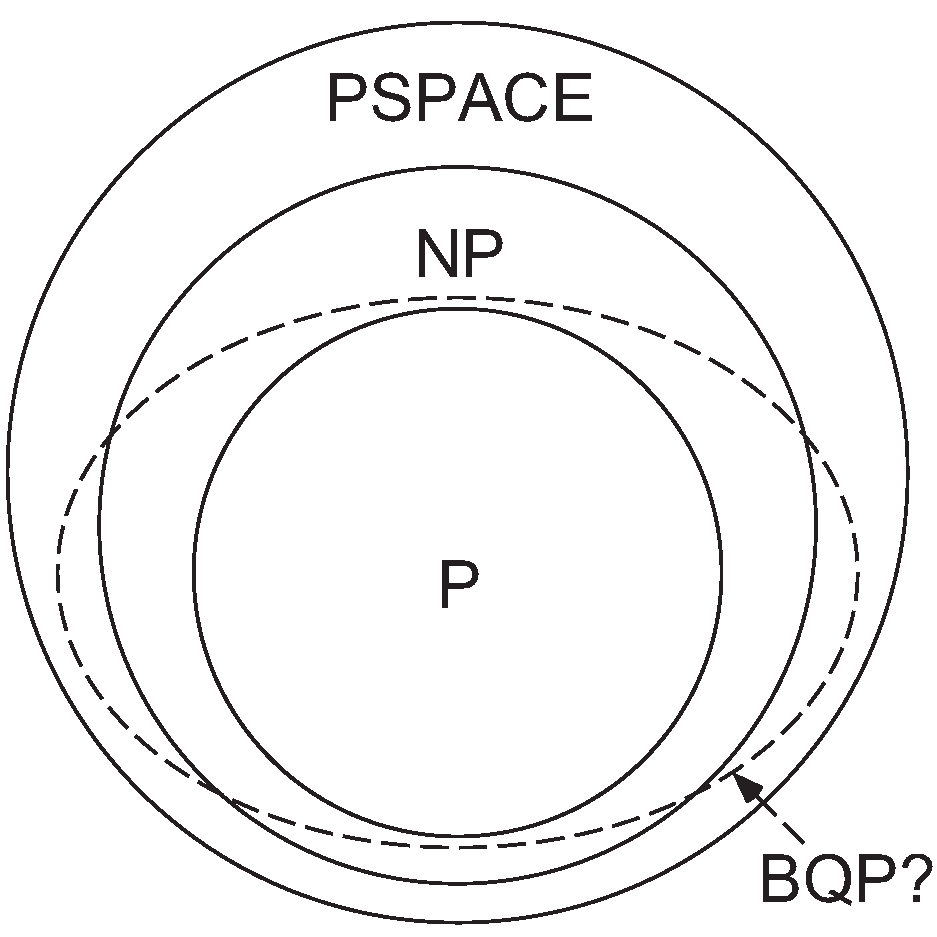
\includegraphics[width=\linewidth]{Quantum-complexity.png}
    \centering
    \caption{Complexity classes hierarchy.}
    \end{figure}